\documentclass{article}
\usepackage{tikz}
\usepackage{pgfplots}
\pgfplotsset{compat=1.8}
\usepgfplotslibrary{statistics}
\begin{document}
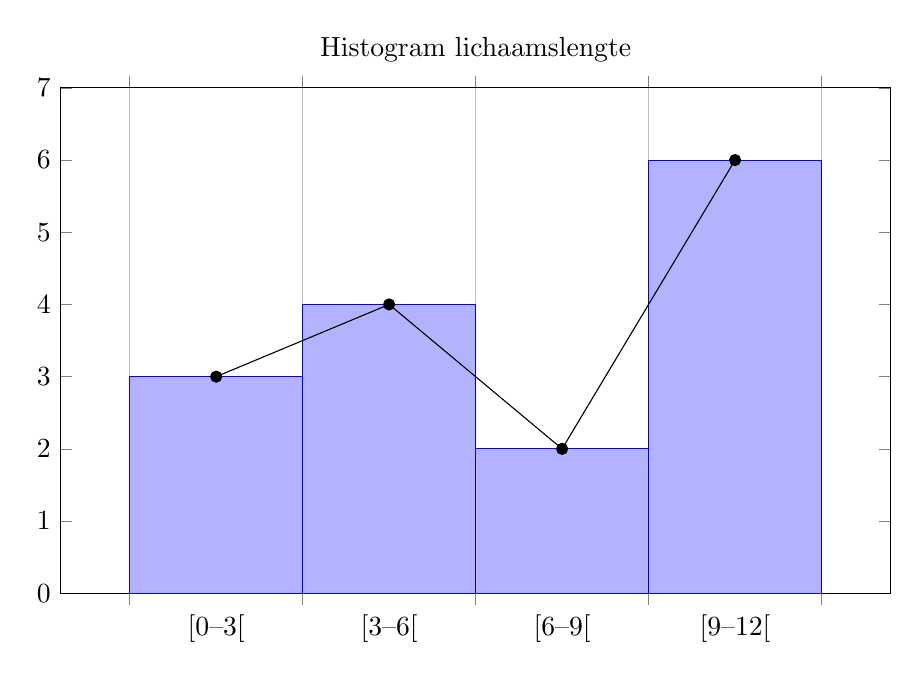
\begin{tikzpicture}
\begin{axis}[
width=1*\textwidth,
height=8cm,
ymin=0,
ymax=7,
title=Histogram lichaamslengte,
ybar interval,
xticklabel={[\pgfmathprintnumber\tick--\pgfmathprintnumber\nexttick [}],
\addplot+[hist={bins=4, data max=12,data min=0}]
table[row sep=\\,y index=0] {
data\\
1\\ 2\\ 1\\ 5\\ 4\\ 10\\ 4\\ 5\\ 7\\ 10\\ 9\\ 8\\ 9\\ 9\\ 11\\
};

\addplot[
	%
	mark=*,
	hist={bins=4, data max=12,data min=0,
		% this here should *not* become an ybar interval:
		handler/.style={sharp plot},intervals=false,
	},
	%
	% .. but since the other plot is shown with intervals, we should
	% shift this here accordingly:
	shift={(axis direction cs:1.5,0)},
]
table[row sep=\\,y index=0] {
data\\
1\\ 2\\ 1\\ 5\\ 4\\ 10\\ 4\\ 5\\ 7\\ 10\\ 9\\ 8\\ 9\\ 9\\ 11\\
};
\end{axis}
\end{tikzpicture} 
\end{document}
